\section{Technique and implementation}
%% \label{sec:approach}

\begin{figure*}
  \centering
  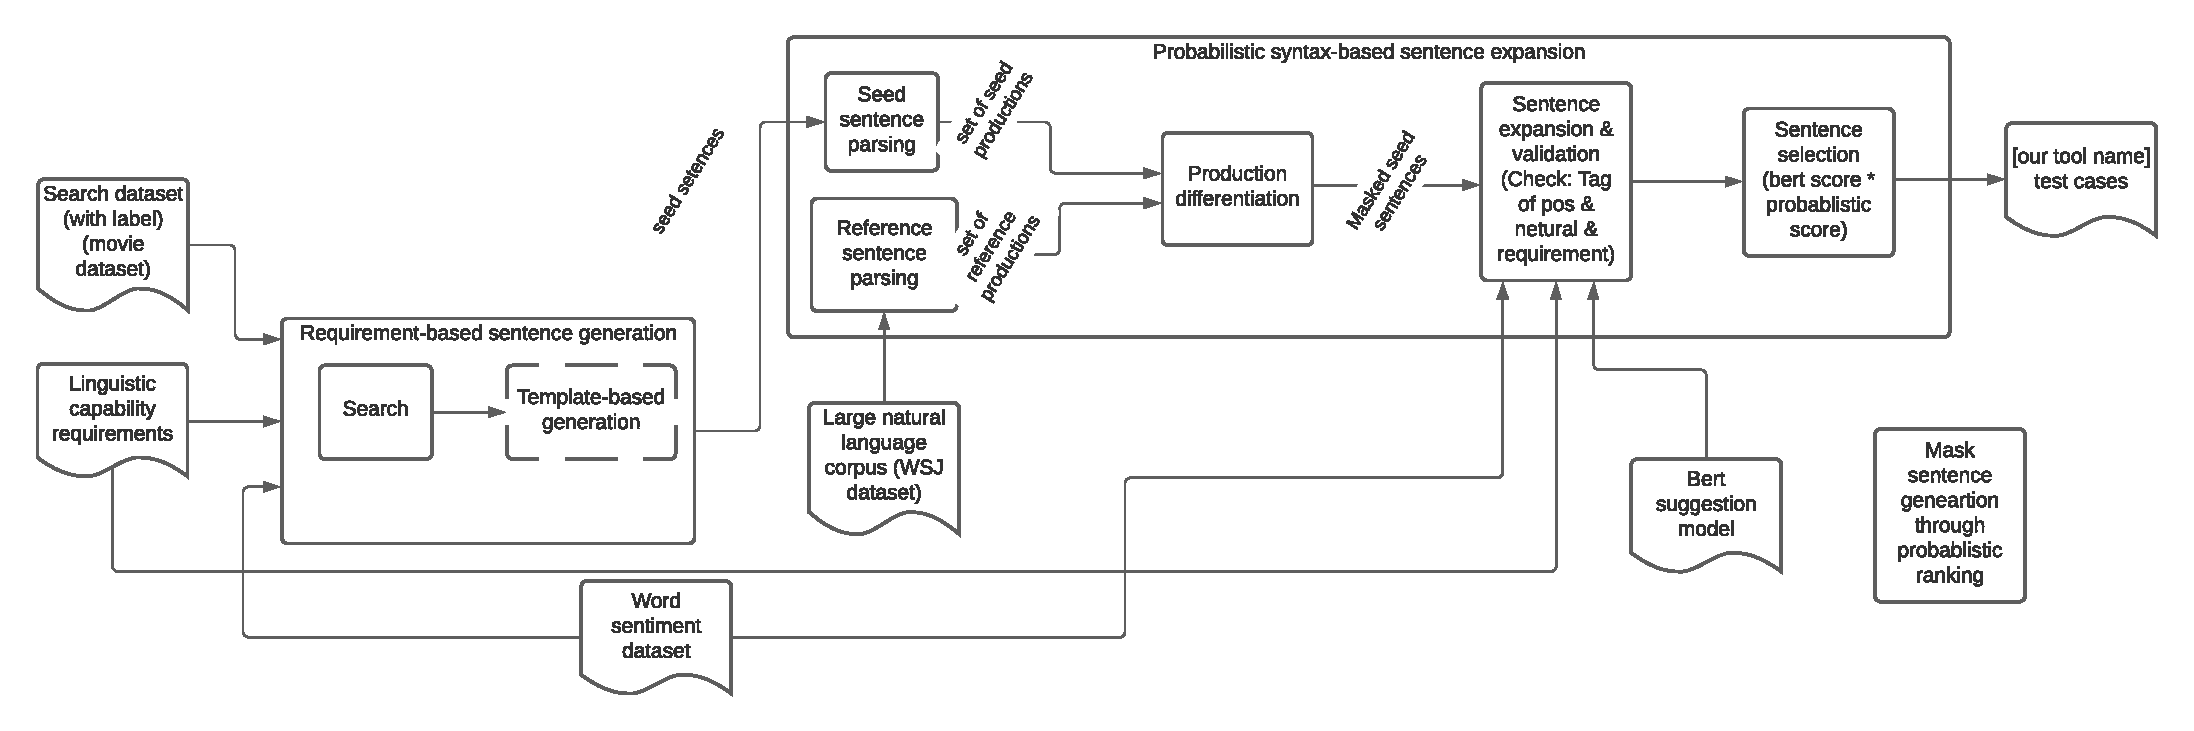
\includegraphics[scale=0.5]{figs/overview.pdf}
  \vspace{-5pt}
  \caption{\OverallModelFigCaption}
  \vspace{-10pt}
\end{figure*}

\Model generates input \sents with the following phases illustrated in
\ref{fig:OverallModel}: 1. search phase searches seed \sents according
to its \req of \lc, 2. seed parsing phase parses the found seed \sents
and extract their \cfg, 3. reference parsing phase collects \pcfg from
large corpus, 4. production differentiation phase identifies
structural expansion candidates for input expansion, and 5.\sent
selection phase generates natural expanded \sent. In this section, we
provide more details on each phase.

\subsection{Search phase}
The search phase in \Model searches inputs in dataset and selects
subset of input \sents in the dataset that meets the \lc
\req. The idea behind this phase is that input distribution of
\lc is important to generate inputs relevant to \lc. \Lc explains
expected behaviors of NLP model on specific types of input and
output. The NLP model is evaluated on how much it performs on the
input and output. Thus, \lc introduces the constraints of the input
data. Input data from the constrained distribution are only qualified
to be used for evaluating the NLP model on the \lc.  In addition,
diversity in inputs is important to evaluate NLP models on the
\lc. Inputs that differ are more likely to cover the NLP model
behavior, and more coverage increases trustworthiness of the
evaluation. To generate inputs from same distribution on \lc and high
diversity of inputs, we estabilish \reqs of input and output
for each \lc, and find inputs that fulfil the \reqs. Given a
\lc, a \req consists of search \req, transform
\req and expansion \req. The search \req
describes features and functionalities that we seek to have in
inputs. \Model check each input if it satisfy the \req.

\begin{figure}[t]
  \centering
  \lstinputlisting[language=json-pretty]{code/requirement_sa1.json}
  \vspace{-10pt}
  \caption{\SearchRequirementExampleFigCaption}
  \vspace{-10pt}
\end{figure}

\begin{figure}[t]
  \centering
  \subfloat[][\TransformRequirementExampleSubFigCaption]{\lstinputlisting[language=json-pretty]{code/requirement_sa2.json}}
  \\
  \subfloat[][\TransformTemplateExampleSubFigCaption]{\lstinputlisting[language=python-pretty]{code/requirement_sa2.py}}
  \\
  \caption{\TransformRequirementExampleFigCaption}
  \vspace{-10pt}
\end{figure}

Figure~\ref{fig:SearchReqEx} shows \lc of \SareqExOne. To evaluate
this \lc, the input is required to be short and have only \neu \adjs,
\neu \nns. In addition, the label needs to be \neu. Therefore, all
short natural \sents with only \neu \adjs and \neu \nns are available
to evaluate NLP models. Next, transform \req explains how the input
and output needs to be tranfromed. Some \lc only accepts heavily
limited input distribution, and it is unlikely to be included in
searching dataset because of its high structural diversity, thus,
finding such \sents is costly. Therefore, our approach is to find
inputs by relaxing search requirement and transform the input to match
the target requirement of the \lc. In this work, the inputs are
transformed by word addition or perturbing the found inputs with \lc
dependent templates. The figure~\ref{fig:TransformReqEx} shows the
example of use of the template requirement. The \lc of \SareqExTwo in
the figure~\ref{fig:TransformReqSubEx} requires inputs to be the
negated \pstv \sents and the neutral expression in the middle. Rather
than searching \sents that match the input distribution of the \lc,
the \Model search \pstv and \neu inputs and combine them into negated
\pstv \sents. Figure~\ref{fig:TransformTempSubEx} illustrates template
for the \lc. According to the \lc, The value of ``sent1'' and
``sent2'' become each searched \neu and \pstv inputs respectively, and
the template completion generates new inputs that matches the target
\lc. In addition, the transformation of inputs also produce high
diversity in the inputs because of that from initially found
inputs. In this paper, we will denote the searched inputs in this
phase as seed inputs.

\subsection{Seed parsing phase}
To expands seed sentence and generate fluent and faithful sentence
used for evaluation, \Model studies structure of each seed input for
its expansion. To extract the structure, this phase takes each seed as
input, and the parse tree of the seed input is output.  In this phase,
\Model implements the Berkeley Neural
Parser~\cite{kitaev2018seedparser,kitaev2019seedparser}.

\subsection{Reference parsing phase}
We take a large scale corpus as reference for seed expansion. It is
motivated by that large corpus represents data distribution of real
world, and the discrepancy between seed and reference leads to
determine how the seed can be expanded within real world data
distribution. This phase builds \pcfg from the reference corpus. \cfg
is constructed by parsing sentences in the corpus and extracting
production rules. In addition, the probability of \cfg is estimated by
its frequency over corpus. The outpus of this phase is the constructed
\pcfg, and it is compared with seed parse trees. For our
implementation, we build the \pcfg from the Penn Treebank corpus dataset.

\subsection{production differentiation phase}
\begin{algorithm}
  \caption{\ProdDiffAlgCaption}
  \begin{algorithmic}[1]
    \State \textbf{Input:} Parse trees of seed sentences $\textbf{S}$,
    reference \pcfg$\textbf{R}$
    \State \textbf{Output:} Set of expanded masked sentences $\textbf{S\_exp}$
    \For {$seed$ from $S$}
      \For {each production rule $seed\_prod$ from $seed$}
        \State $seed\_lhs = seed\_prod.lhs$
        \State $seed\_rhs = seed\_prod.rhs$
        \For {$ref\_rhs$, $ref\_prob$ from $R[seed\_lhs]$}
          \If {$seed\_rhs$ is superset of $ref\_rhs$}
            \State $parent = seed\_prod.parent$
            \State $prob = ref\_prob$
            \While {$parent$ is not empty}
              \For {$par\_rhs$, $par\_prob$ from $R[parent.lhs]$}
                \If {$parent.rhs == par\_rhs$}
                  \State $prob = prob \cdot par\_prob$
                  \State $parent = parent.parent$
                  \State break
                \EndIf
              \EndFor  
            \EndWhile
            \State $P.add([seed\_prod, ref\_prod, prob])$
          \EndIf
        \EndFor
      \EndFor
      \If {$P$ is not empty}  
        \State Select Top-k $ref\_prod$ along with probabilities in P
        \For {each $seed\_prod$, $ref\_prod$ in the Top-k selected P}
          \State replace $seed\_prod$ with $ref\_prod$ in $seed$
          \State replace expanded component in $ref\_prod$ with $MASK$
          token in $seed$ sentence
          \State $S\_exp.add([ref\_prod, expanded sentence])$
        \EndFor
      \EndIf
    \EndFor
  \end{algorithmic}
\end{algorithm}


Given the seed parse tree and reference \pcfg, production
differentiation phase suggests structural expansion candidates on the
seed input. this phase aims to analyze which structural components and
where they can be added into the seed structure for its expansion. To
do so, we explore reference production rules comparing it with each
production rule used in seed input. This results in the phase
described in Algorithm~\ref{code:ProdDiffAlg}. For each production
rule in seed inputs ($seed\_prod$), it searches production rules in
reference ($ref\_prod$) which it has same non-terminal on the
left-hand side ($seed\_prod.lhs==ref\_prod.lhs$) and superset of
right-hand side of the seed production rule ($seed\_prod.rhs \subset
ref\_prod.rhs$).  As we assume that the reference \cfg is built from
real world data distribution, the elements in the complement set
($ref\_prod.rhs - seed\_prod.rhs$) become an expansion candidate which
can be expanded from the $seed\_prod.rhs$ found in real world. In
addition, the measure of how consistent the production rule is with
the given seed structure is given in its probability of the reference
production rule ($ref\_prob$) multiplied by that of parents of
$seed\_prod$. The expansion candidate consists of terminal or
nonterminal symbols. When there is a phrase-level or clause-level
nonterminal symbol, \eg noun phrase, it needs to be expanded and
replaced with word-level nonterminal or terminal symbols to generate
the expansion candidate. The number of feasible replacement is
unbounded because of its high degree of freedom. Therefore, in this
work, we focus on the expansion candidate with only the word-level
nonterminal or terminal symbols for the effectiveness of \Model.

\subsection{\Sent selection phase}

